\chapter{Mechanik}

\section{Kinematik}
Beschreibung von Bewegungen \\
einfachster Fall:
\begin{itemize}
	\item geradlinige Bahn (1D)
	\item gleichförmige Bewegung
\end{itemize}
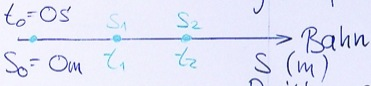
\includegraphics{Bild1}

\subsection{Weg-Zeit-Diagramm}
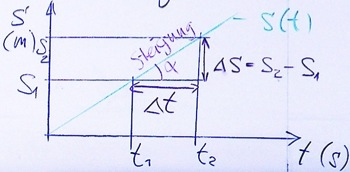
\includegraphics{Bild2}
\[ \tan \alpha = \frac{\Delta s}{\Delta t} \overset{!}{=} v \]
konst. Steigung von $s(t) \implies$ konst. $v$

\subsection{Geschwindigkeit}
\begin{def*}[ note = Geschwindigkeit , index = Geschwindigkeit ]
	\[
		v = \frac{\Delta s}{\Delta t} \\
		[v] = \frac{m}{s}
	\]
\end{def*}

\subsection{Geschwindigkeits-Zeit Diagramm}
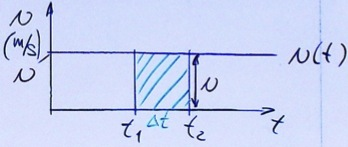
\includegraphics{Bild3}
\[
	v(t) = \frac{\Delta s}{\Delta t} \\
	\text{Fläche} = v \cdot \Delta t = \Delta s \text{ ! } = \text{ zurückgelegter Weg}
\]

\subsection{Nicht-gleichförmige Bewegungen}
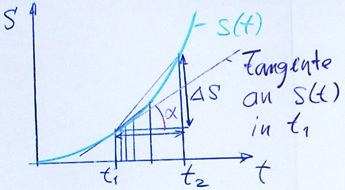
\includegraphics{Bild4}
Geschwindigkeit $v(t)$
\[
	\overline{v} = \frac{\Delta s}{\Delta t} = \text{ mittlere Geschwindigkeit zw. $t_1$ und $t_2$} \\
	v(t_1) = \lim_{t_1 \rightarrow t_2} \frac{\Delta s}{\Delta t} \underset{\text{\scriptsize{Math.}}}{=} s'(t) \\
	v(t) = s'(t) \\
\]

\subsubsection{Schreibweise}
\[
	\Delta t \rightsquigarrow \dd t \\
	v(t) = s'(t) \eqqcolon \frac{\dd s}{\dd t}
\]
1. Ableitung \\
$v(t)$: Momentangeschwindigkeit
\begin{bsp*}[ note = $v$ nimmt gleichmässig zu ]
	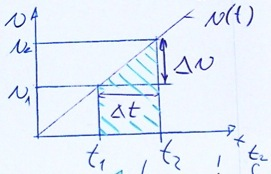
\includegraphics{Bild5}
	\[ \text{Fläche } \underset{\text{\scriptsize{Math.}}}{\overset{\text{!}}{=}} \int_{t_1}^{t_2} v(t) \dd t \]
\end{bsp*}
\todo{Undefined seq.}
Änderung der Geschwindigkeit mit der Zeit:
\begin{def*}[ note = Beschleunigung , index = Beschleunigung ]
	\[
		a = \frac{\Delta v}{\Delta t} \\
		[a] = \frac{m}{s^2}
	\]
\end{def*}
Fall:
\begin{itemize}
	\item gleichförmige Beschleunigung: $a =$ konst.
	\item beliebige Funktion $a(t)$
\end{itemize}
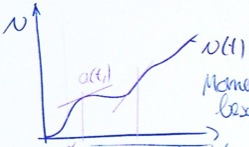
\includegraphics{Bild6} \\
analog:
\[
	a(t) = \frac{\dd v}{\dd t} \\
	a(t) = \frac{\dd}{\dd t} \left( \frac{\dd s}{\dd t} \right) = s''(t) \eqqcolon \frac{\dd^2 s}{\dd t^2}
\]

\begin{rep*}[note = Kinematik (1D-Fall)]
	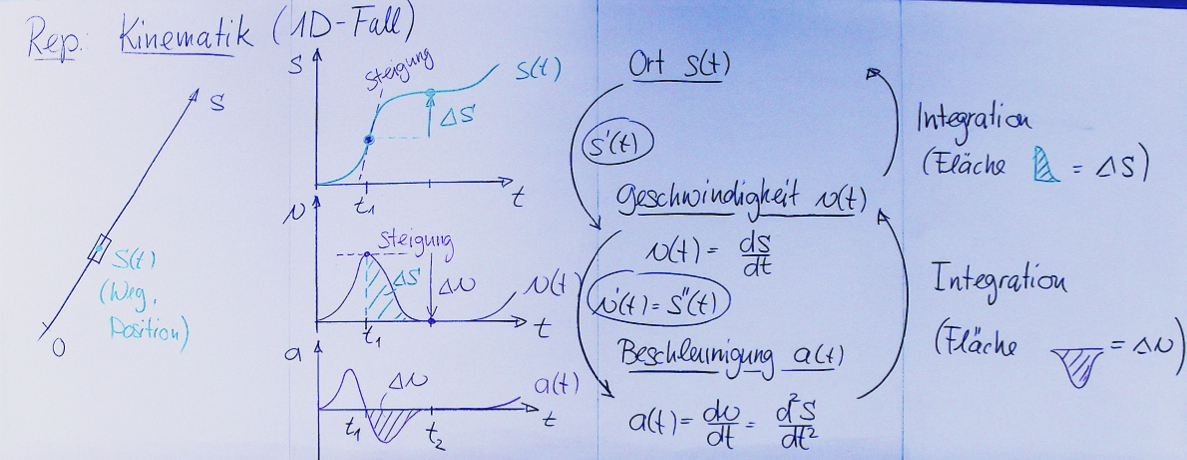
\includegraphics[ width = \textwidth ]{Bild7}
\end{rep*}
\begin{bsp*}[note = Der freie Fall]
	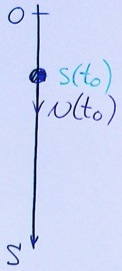
\includegraphics{Bild8} \\
	auf der Erdoberfläche
	\[ a(t) = a_{\text{Fall}} = g = 9.81 \frac{\text{m}}{{\text{s}}^2} \]
	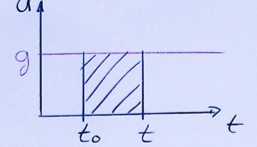
\includegraphics{Bild9}
	\[ \text{Fläche } = g( t - t_0 ) \]
	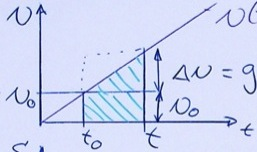
\includegraphics{Bild10}
	\[
		v(t) = v_0 + g( t - t_0 ) \\
		\Delta v = g( t - t_0 ) \
		\text{Fläche } = v_0 ( t - t_0 ) + \frac{1}{2} g( t - t_0 )^2 = \Delta S
	\]
	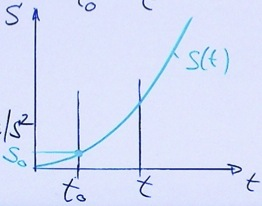
\includegraphics{Bild11}
	\[ s(t) = s_0 + v_0 ( t - t_0 ) + \frac{1}{2} g( t - t_0 ) \]
	
	einfachster Fall:
	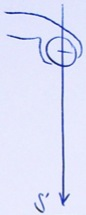
\includegraphics{Bild12}
	\[
		s(0) = 0 \\
		t_0 = 0 \\
		s_0 = 0 \\
		v_0 = 0 \\
		\implies s(t) = \frac{1}{2} gt^2
	\]
\end{bsp*}

\subsection{Bewegungen in der Ebene}
\subsubsection{Ortsvektor \texorpdfstring{$\vec{r}(t)$}{r(t)}}
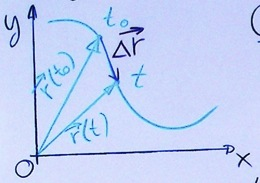
\includegraphics{Bild13}
\begin{itemize}[label = $\rightarrow$]
	\item Länge (Betrag)
	\item Richtung
\end{itemize}

Geschwindigkeit: $\frac{\text{Weg}}{\text{Zeit}}$
Weg: $\Delta \vec{r} = \vec{r}(t) - \vec{r}(t_0)$ \\
$\vec{v} = \frac{\Delta \vec{r}}{\Delta t}$ mittlere Geschwindigkeit \\
Momentangeschwindigkeit: $\vec{v}(t) = \lim_{\Delta t \rightarrow 0} \frac{\Delta \vec{r}}{\Delta t} \overset{\text{\scriptsize{Math.}}}{=} \frac{\dd \vec{r}}{\dd t}$ \\
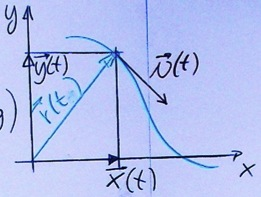
\includegraphics{Bild14}
\[
	\vec{r}(t) = \vec{x}(t) + \vec{y}(t) \\
	\implies \text{ Komponentenschreibweise} \\
	\vec{r}(t) = ( x(t) , y(t) ) \\
	\frac{\dd \vec{r}}{\dd t} = \left( \frac{\dd x}{\dd t} , \frac{\dd y}{\dd t} \right)
\]
$v(t)$:
\begin{itemize}
	\item Betrag (Schnelligkeit)
	\item Richtung! (tangential zu Bahn)
\end{itemize}
\subsubsection{Schnelligkeit}
\[ \abs{\vec{v}(t)} = v(t) = \sqrt{{v_1}^2(t) + {v_2}^2(t)} \]
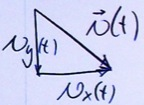
\includegraphics{Bild15}

\subsubsection{Momentanbeschleunigung}
\[ \vec{a}(t) = \frac{\dd \vec{v}}{\dd t} = \frac{\dd^2 \vec{s}}{\dd t^2} \]

\subsection{Wann ist eine Bewegung beschleunigt?}
Wenn $\vec{v}$ sich ändert!
\begin{itemize}[label = $\rightarrow$]
	\item Betrag
	\item Richtung!
\end{itemize}
\begin{bsp*}[note = Kreisbewegung mit konstante Umlaufgeschwindigkeit]
	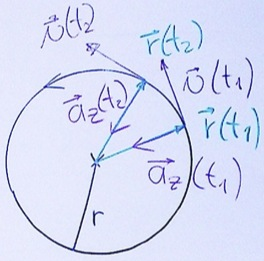
\includegraphics{Bild16}\\
	$\implies v =$ konst., $\vec{v}$ dreht $\implies$ Zentripetalbeschleunigung
	\[ a = \frac{v^2}{r} \]
\end{bsp*}
\begin{bsp*}[note = beliebige Kreisbewegung ($v \neq$ konst.)]
	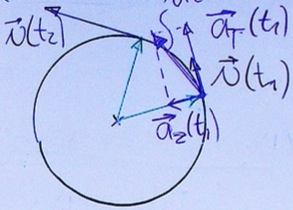
\includegraphics{Bild17} \\
	\[ \begin{matrix*}[l]
		a_Z(t) = \frac{v^2(t)}{r}		&\text{Zentripetalbeschleunigung} \\
		a_T(t) = \frac{\dd v}{\dd t}	&\text{Tangentialbeschleunigung}
	\end{matrix*} \]
\end{bsp*}

\subsection{Bewegungen im 3D-Raum}
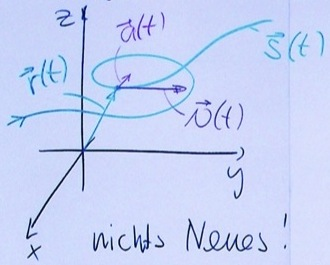
\includegraphics{Bild18} \\
nicht Neues!
\[ \vec{r}(t) = ( x(t) , y(t) , z(t) ) \]
